
%%%%%%%%%%%%%%%
%     IMPLEMENTATION     %
%%%%%%%%%%%%%%%

\begin{figure}
\centering
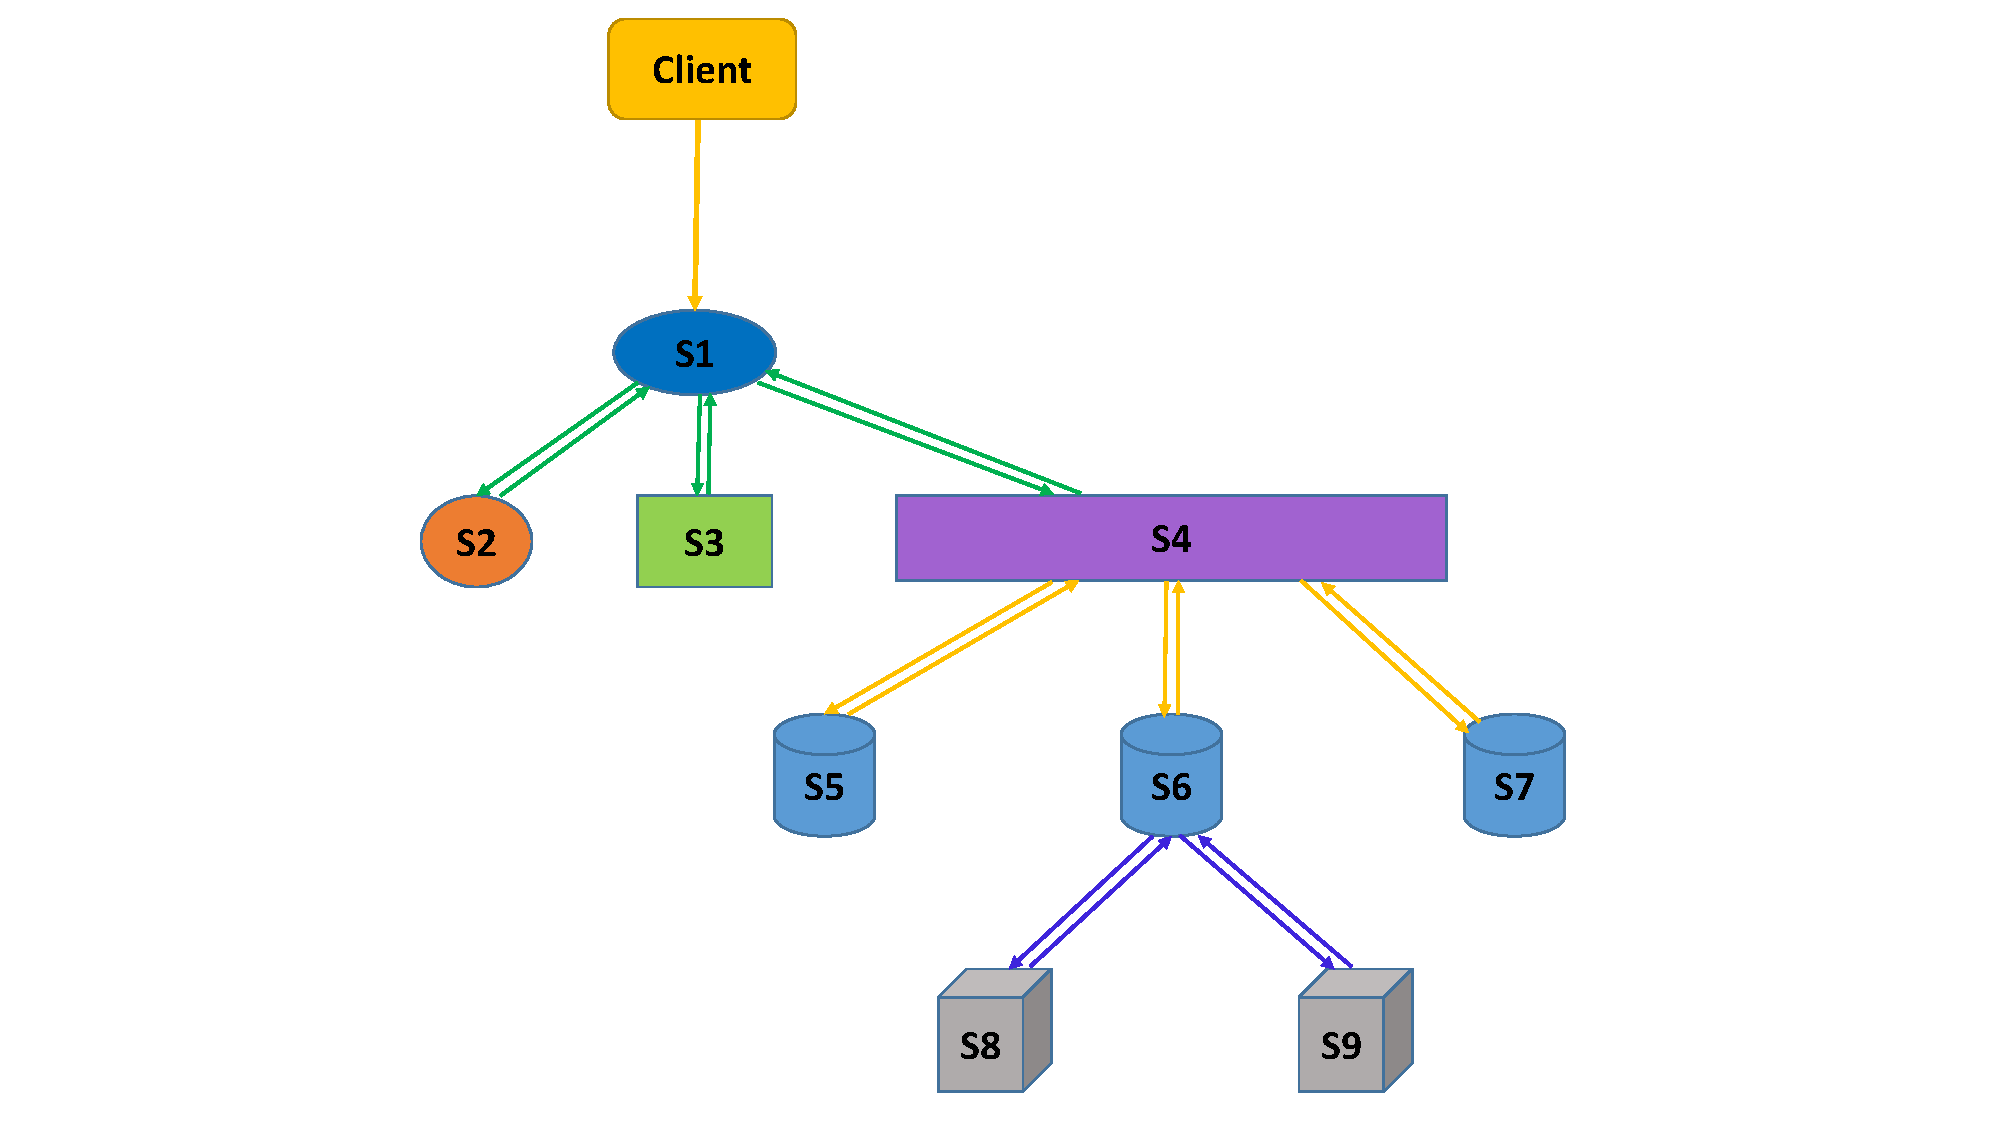
\includegraphics[width=8cm,height=10cm,keepaspectratio=true]{toy_architecture}
\caption{Test architecture consisting of a small set of microservices}
\label{toy_arch}
\end{figure}


\section{Implementation} \label{implementation}
This section details the implementation choices that we have chosen to pursue to build our framework. Because we do not have a real microservice architecture to perform tests on, we built a simple service consisting of two \textbf{servers} listening on two different ports and a set of services contained in each server, the architecture of which can be seen in Figure \ref{toy_arch}. The services are coded to construct spans upon being called, and will provide detailed traces of their states. The \textbf{client} will start by invoking service1 on the first server, which will trigger the full call graph and provide the complete trace.

We chose \textbf{golang}\cite{google:golang} as our programming language because of its extensive support for the Opentracing framework and because of the strength of its \textbf{decorator} syntax. In total, the lines of code is just shy of 500 lines including the code for the servers, client, and the fault handling mechanism. The wire protocol chosen was \textbf{HTTP} in the form of REST method calls, and support provided by Golang made it very easy to integrate a decorator that wraps around all of the services. 

We leverage the powerful \textbf{Baggage} annotation provided by Opentracing to propagate our failures downstream. The client can accept as argument any service that it wants to target for failure testing, and will inject a baggage item whose key serves as a flag into its own span. This baggage is then propagated to whichever service that it calls, and further downstream if the said service calls upon other services all of which can see the client span's baggage items. Because we have decorated our handler to intercept service calls, our decorator will detect if the failure flag exists before proceeding to calling the service itself. If the flag exists, and the decorator notices that the service at hand matches that which has been signaled for failure, then it will act and perform the injection. 

Two of the most common types of failures in distributed services are \textit{unknown delays} and \textit{packet lost}. When services send data to one another, we can never be certain when, or if, the data will arrive. In our implementation, we allow the tester to specify the delay time to see how the upstream services react, and the decorator will simply sleep for this duration before calling the service itself. To simulate packet lost, we have the decorator ignore the request and never actually call the service. 

The verification step to see if our fault injection does work as intended is fairly straightforward. To verify that a delay is actually injected, we simply check that a service's span traces will be delayed for said period of time before being printed. To verify that a packet has indeed been dropped, we check that the service's span traces is not printed along with the other spans' traces.


%%%%%%%
%    EOF     %
%%%%%%%